\documentclass[onlytextwidth,usepdftitle=false]{beamer}
\mode<presentation>

\hypersetup{pdftitle={Adaptive Hashing}}
\usepackage[symbol]{footmisc}
\usepackage{adforn}
\usepackage{xpatch}
\usepackage{svg}


%% Algorithms

\usepackage{algorithm}
\usepackage[noend]{algpseudocode}
\usepackage{algorithmicx}
\newcommand*\Let[2]{\State #1 $\gets$ #2}
\algdef{SE}[DOWHILE]{Do}{doWhile}{\algorithmicdo}[1]{\algorithmicwhile\ #1}%
\algrenewcommand\algorithmicindent{1em}%


%% Math

%https://tex.stackexchange.com/questions/512903/how-can-i-use-shorter-minus-signs-in-math-subscripts
\DeclareMathSymbol{\shortminus}{\mathbin}{AMSa}{"39}
\newcommand\var[1]{\mathit{#1}}
\newcommand\fn[1]{\operatorname{#1}}


%% Language
\usepackage[UKenglish]{babel}
\renewcommand\UKenglishhyphenmins{22}
\frenchspacing
%https://tex.stackexchange.com/a/44669
\usepackage{ragged2e}
\let\raggedright=\RaggedRight


%% Microtype

\usepackage{ifxetex}
\ifpdftex
  \usepackage[spacing=true]{microtype}
\else
  \usepackage{microtype}
\fi


%% Font

%% \usepackage[sc]{mathpazo}
%% \usepackage[parindent=0pt,fontsize=9.59pt]{fontsize}
%% \newcommand{\titlefont}{}

%% % Times New Roman font, pdflatex
%% \RequirePackage[p,osf]{newtx}
%% \newcommand{\titlefont}{}
%% \usepackage[parindent=0pt,fontsize=11pt]{fontsize}

%% % Utopia
%% \RequirePackage[p,osf,semibold,scaled=1.0781548]{ebgaramond}
%% \RequirePackage{utopia}
%% \RequirePackage[parindent=0pt,fontsize=10.102pt]{fontsize}
%% \newcommand{\titlefont}{}
%% \newcommand{\titleliningnums}[1]{{\liningnums{#1}}}
%% \color{gray!190}

%% \usepackage{librebaskerville}
%% \newcommand{\titlefont}{}
%% \usepackage[parindent=0pt,fontsize=9.0pt]{fontsize}
%% \linespread{1.1}

% XCharter + EB Garamond
\ifpdftex
  % With pdflatex, otfmath is not supported.
  \usepackage[p,scosf]{XCharter}
  \usepackage[charter,smallerops,varbb,scaled=1.05]{newtxmath}
  \usepackage[cal=cm]{mathalfa}
  % (* (/ 13.5 12) (/ 11.2265 12)) = 1.0524843
  \usepackage[p,osf,scaled=1.0524843]{ebgaramond}
\else
  \usepackage[no-math]{fontspec}
  % (* (/ 13.5 12) (/ 11.2265 12)) = 1.0524843
  \usepackage[p,osf,scaled=1.0524843]{ebgaramond}
  \usepackage[xcharter,p,osdf,scosf,smallerops,varbb,mathscale=1.05]{newtx}
\fi
\newcommand{\titlefont}{\ebgaramond}
\usepackage{letltxmacro}
\LetLtxMacro\titleliningnums\liningnums
%% 11.2265 XCharter is equivalentish to 12pt Times.
%% (* 11/12 11.2265) => 10.290958 is thus equivalent to 11pt.
\usepackage[parindent=0pt,fontsize=9.355416pt]{fontsize}
\newcommand\inlinett[1]{\texttt{\fontsize{10pt}{12pt}\selectfont #1}}
\linespread{1.1}

%% % Default
%% \usepackage[parindent=0pt,fontsize=10pt]{fontsize}
%% \newcommand{\titlefont}{}

%% % Libertinus font
%% \usepackage[p,osf]{libertinus}
%% \usepackage[libertine,vvarbb]{newtxmath}
%% \let\openbox\relax
%% \newcommand{\titlefont}{}
%% \usepackage[parindent=0pt,fontsize=10pt]{fontsize}
%% \linespread{1.1}

%% \usepackage{fourier}
%% \usepackage{plex-serif, plex-mono}
%% \usepackage[sfdefault]{plex-sans}
%% \newcommand{\titlefont}{}
%% \usepackage[parindent=0pt,fontsize=8.16pt]{fontsize}
%% \linespread{1.1}

%% % Cochineal = Recent Crimson font (=Amari?) with fixes, extensions
%% \usepackage[p,osf]{cochineal}
%% \usepackage[parindent=0pt,fontsize=10.56pt]{fontsize}
%% \usepackage[varqu,varl,var0,scale=0.93]{inconsolata}
%% \usepackage[scale=.95,type1]{cabin}
%% \usepackage[cochineal,vvarbb]{newtxmath}
%% \usepackage[cal=boondoxo]{mathalfa}
%% \let\openbox\relax
%% % (/ 12.67603 13.23523 1.02) = 0.93896973
%% \usepackage[p,osf,scaled=0.93896973]{ebgaramond}
%% \newcommand{\titlefont}{\ebgaramond}
%% \newcommand{\titleliningnums}[1]{{\liningnums{#1}}}

%% Kerning of EB Garamond smallcaps in some titles

\newcommand\Adaptive{Ad\hspace{-0.06em}aptive}
\newcommand\Hashing{Hashin\hspace{-0.02em}g}
\newcommand\Motivation{Motiv\hspace{-0.06em}a\hspace{-0.03em}tion}


%% Color

\definecolor{titlepagebg}{RGB}{35,31,32}
\definecolor{titlepagefg}{RGB}{229,225,226}
\definecolor{titlepagefg2}{RGB}{190,190,190}
\definecolor{mglred}{RGB}{154,60,45}
\definecolor{mglred2}{RGB}{131,51,39}

\colorlet{mygrey}{black!50!white}
\colorlet{mygreen}{green!50!black}
\colorlet{myblue}{blue!70!black}
\colorlet{myorange}{orange!70!white}
\colorlet{myred}{red!70!black}


%% Layout

\newcommand\setlengths{%
  \setlength{\parskip}{1\baselineskip}%
  \setlength{\topsep}{0\baselineskip}%
  \setlength{\parsep}{0.25\baselineskip}%
  \setlength{\partopsep}{0\baselineskip}}
\setlengths
%https://tex.stackexchange.com/questions/225736/latex-beamer-define-itemsep-globally
\xpatchcmd{\itemize}
  {\def\makelabel}
  {\setlength{\topsep}{0\baselineskip}
   \setlength{\parskip}{0.5\baselineskip}
   \setlength{\partopsep}{0.5\baselineskip}
   \setlength{\parsep}{0.5\baselineskip}
   \setlength{\itemsep}{0\baselineskip}
   \def\makelabel}
  {}
  {}
\newcommand\toplevellist{%
  \settowidth{\leftmargini}{\usebeamertemplate{itemize item}}
  \addtolength{\leftmargini}{\labelsep}}
\newcommand\looselist{\setlength{\parskip}{1\baselineskip}}
%https://tex.stackexchange.com/questions/338592/beamer-set-global-parskip-for-all-columns
\makeatletter
\newcommand{\@minipagerestore}{\setlengths}
\makeatother
\setbeamersize{text margin left=2\baselineskip}
\setbeamersize{text margin right=2\baselineskip}
\newcommand\figurecolumn{%
  \footnotesize%
  \vspace{1\baselineskip}%
  \setlength{\parskip}{0.2\baselineskip}}


%% Beamer styling

\usefonttheme{serif}
\setbeamerfont{author}{size=\large,family=\titlefont}
\setbeamercolor{author}{fg=titlepagefg2}
\setbeamerfont{institute}{size=\footnotesize,family=\titlefont}
\setbeamercolor{institute}{fg=titlepagefg2}
\setbeamercolor{date}{fg=titlepagefg2}
\setbeamerfont{date}{size=\small,family=\titlefont}
\setbeamercolor{title}{fg=mglred2}
\setbeamerfont{title}{shape=\scshape,family=\titlefont}
\setbeamercolor{subtitle}{fg=black}
\setbeamerfont{subtitle}{shape=\scshape,family=\titlefont}
\setbeamercolor{section in toc}{fg=black}
\setbeamerfont{section in toc}{shape=\scshape}
\setbeamercolor{frametitle}{fg=mglred2}
\setbeamerfont{frametitle}{shape=\scshape,family=\titlefont}
\setbeamercolor{itemize item}{fg=mglred2}
\setbeamercolor{enumerate item}{fg=mglred2}
\setbeamertemplate{itemize item}{\raisebox{0.1em}{\scalebox{0.75}{$\bullet$}}}
\setbeamertemplate{navigation symbols}{}


%%%% Tikz and Pgfplots

\usepackage{tikz}
\usepackage{pgfplots,tikz,pgfplotstable}
\usepackage{pgfornament}
\pgfplotsset{compat=1.9}
\usetikzlibrary{positioning, fit, arrows.meta, shapes, chains, scopes}
\usetikzlibrary{backgrounds, shapes.geometric, shapes.multipart}
\usetikzlibrary{shapes.geometric, arrows, decorations, decorations.text}

\usetikzlibrary{external}
\tikzexternalize[prefix=tikz/]
%% \tikzset{external/optimize command away=\AddToShipoutPictureBG}

%https://tex.stackexchange.com/questions/84127/correctly-align-vertical-text-on-a-baseline-in-pgfplots
\def\mystrut{\vphantom{hg}}
%https://tex.stackexchange.com/questions/204395/add-custom-entry-into-legend-in-pgfplot
\pgfplotsset{
    legend image with text/.style={
        legend image code/.code={%
            \node[anchor=center] at (0.3cm,0cm) {#1};
        }
    },
}
\pgfplotsset{every axis/.append style={
    ticklabel style = {font=\scriptsize},
    ylabel shift = -0.25\baselineskip
}}
\pgfplotsset{uniformhash/.style = {mygrey, loosely dotted, thick}}
\pgfplotsset{murmurhash/.style = {mygreen, densely dotted, line width=0.8pt}}
\pgfplotsset{prefuzzhash/.style = {myblue, densely dashed, line width=0.6pt}}
\pgfplotsset{constanthash/.style = {myorange, densely dashdotted, thick}}
\pgfplotsset{adaptivehash/.style = {myred, line width=0.5pt}}


%% Content commands
\newcommand*\lisp[1]{\inlinett{#1}}

\colorlet{uniformhashcolor}{mygrey}
\colorlet{murmurhashcolor}{mygreen}
\colorlet{prefuzzhashcolor}{myblue}
\colorlet{constanthashcolor}{myorange}
\colorlet{adaptivehashcolor}{myred}

\newcommand\mglconclusion[1]{\textcolor{mglred2}{\textbf{\maltese} #1}}
\newcommand\lispersonly[1]{}
%% \newcommand\lispersonly[1]{#1}


\title{\vspace{0.5\baselineskip}\\\textls[150]{AD\hspace{-0.05em}APTIVE\hspace{0.2em} HASHIN\hspace{-0.025em}G}}
\subtitle{\vspace{0.15\baselineskip}\textls[100]{F\hspace{-0.06em}aster Hash Fun\hspace{-0.02em}ctio\hspace{-0.035em}n\hspace{-0.02em}s with Fe\hspace{-0.022em}wer Co\hspace{-0.035em}llisio\hspace{-0.035em}n\hspace{-0.022em}s}\footnote[1]{\tiny {\titlefont \scshape \dots Especially in Certain Situations}}}
\author[G. Melis]{\textit{\textcolor{mglred}{Gábor Melis}} \\[-0.25\baselineskip]
  \inlinett{\scriptsizer melisgl@google.com}
  \\[\baselineskip]
  \href{https://quotenil.com/about-me.html}{%
    
\includegraphics[height=1.7\baselineskip]{die-low-contrast.png}}
}
\institute[GDM]{Google DeepMind}
\date{2024-05-14}


\begin{document}

{
\setbeamercolor{background canvas}{bg=titlepagebg}
\setbeamercolor{title}{fg=titlepagefg}
\setbeamerfont{title}{size=\larger}
\setbeamercolor{subtitle}{fg=titlepagefg2}
\setbeamercolor{normal text}{fg=titlepagefg2}
\setbeamerfont{normal text}{family=\titlefont}
\setbeamerfont{footnote mark}{size=\tiny,family=\titlefont}
% Ineffective. Maybe related to
%https://tex.stackexchange.com/questions/21741/how-do-i-change-footnote-font-size-in-beamer-presentation
\setbeamerfont{footnote}{size=\tiny,family=\titlefont}
\def\footnoterule{}
\begin{frame}[plain]
  \titlepage
\end{frame}
}

\begin{frame}
\frametitle{Outline}
% Overlay and tikzexternalize conflict
\tikzset{external/export next=false}
\begin{tikzpicture}[overlay, remember picture]
\node[] at (current page.south east) [anchor = south east, yshift=-7cm]
{
  \href{https://en.wikipedia.org/wiki/Service_stripe}%
       {
\includegraphics[width=0.7\textwidth]{hash-mark.jpg}}
};
\end{tikzpicture}
\vspace{-2\baselineskip}
\toplevellist
\begin{itemize}
\looselist
\item Motivation: performance in theory and practice
\item The general idea of adaptive hashing
\item Adaptive \lisp{eq} hashing
\item Adaptive \lisp{equal} hashing
\item Wrapping up
\end{itemize}
\end{frame}

\begin{frame}[fragile]
\frametitle{\Motivation}
Hash tables are the most common non-trivial data structure.

\toplevellist
\begin{itemize}
\looselist
\item up to 50\% of the time in a complex database query
\item 2\% of all Google CPU usage
\end{itemize}
\pause
\vspace{0.5\baselineskip}
\begin{tikzpicture}[%scale=.2,
  node distance = 7mm and 4mm,
  start chain = going right,
  arr/.style = {semithick, -Stealth},
  dot/.style = {circle, fill, inner sep=1.2pt,
    label=left:#1},
  every label/.append style = {font=\footnotesize, align=center,
    inner sep=1pt},
  E/.style = {ellipse, draw, fill=#1},
  mpnh/.style = {rectangle split, rectangle split horizontal,
    rectangle split parts=2, draw, fill=gray!20,
    inner sep=2pt, on chain, font=\footnotesize},
  mpnv/.style = {rectangle split, rectangle split parts=8,
    rectangle split part fill={gray!30,gray!10,gray!30,gray!30,gray!30,
      gray!10,gray!30,gray!10},
    draw, minimum height=2ex, font=\footnotesize},
  sym/.style = {yshift=-1mm},
  syp/.style = {yshift=+1mm},
                        ]
\node[mpnv, label=$m$ buckets] (H)
    {\nodepart{one}     \phantom{$k_1$}
     \nodepart{two}     \phantom{$k_1$}
     \nodepart{three}   \phantom{$k_1$}
     \nodepart{four}    \phantom{$k_1$}
     \nodepart{five}    \phantom{$k_1$}
     \nodepart{six}     \phantom{$k_1$}
     \nodepart{seven}   \phantom{$k_1$}
     \nodepart{eight}   \phantom{$k_1$}
    };
\node[right=of H.one east, xshift=-1em] {\footnotesize $\substack{(chaining)\\ \overbrace{\phantom{MMMMMMMMMMMMMMMM}}}$};
%
\node[mpnh, right=of H.two east] (A1) {
  \nodepart{one} $k_1$\vphantom{$kv$}
  \nodepart{two} $v_1$\vphantom{$kv$}
};
\node[mpnh] (A2) {
  \nodepart{one} $k_4$\vphantom{$kv$}
  \nodepart{two} $v_4$\vphantom{$kv$}
};
%
\node[mpnh, right=of H.six east] (B1) {
  \nodepart{one} $k_5$\vphantom{$kv$}
  \nodepart{two} $v_5$\vphantom{$kv$}
};
\node[mpnh] (B2) {
  \nodepart{one} $k_2$\vphantom{$kv$}
  \nodepart{two} $v_2$\vphantom{$kv$}
};
\node[mpnh] (B3) {
  \nodepart{one} $k_6$\vphantom{$kv$}
  \nodepart{two} $v_6$\vphantom{$kv$}
};
%
\node[mpnh, right=of H.eight east] (C1) {
  \nodepart{one} $k_3$\vphantom{$kv$}
  \nodepart{two} $v_3$\vphantom{$kv$}
};
%% arrows (right)
\draw[arr] (H |- H.two east) edge (A1)
           (H |- H.six east) edge (B1)
           (H |- H.eight east) -- (C1)
           ;
\draw[arr] (A1) edge (A2)
           (B1) edge (B2)
           (B2) edge (B3)
           ;
%% dots, ellipses
\node (k1) [dot=$k_1$] at (-28.5mm, 2.5mm) {};
\node (k2) [dot=$k_2$] at (-45mm, 1mm) {};
\node (k3) [dot=$k_3$] at (-40mm, -5mm) {};
\node (k4) [dot=$k_4$] at (-30mm, -6mm) {};
\node (k5) [dot=$k_5$] at (-35mm, -14mm) {};
\node (k6) [dot=$k_6$] at (-50mm, -9mm) {};


\scoped[on background layer]
{
\draw[fill=gray!30] (-4,0) circle[radius=2.25];
\path [postaction={
    decoration={
      text along path,
      text format delimiters={|}{|},
      text={|\footnotesize|Universe of keys},
      text align=fit to path,
      reverse path
    },
    decorate
}] (-4,0)++(55:2.0) arc (55:125:2.0);

\draw[fill=white]   (-4,-0.4) circle[radius=1.6];
\path [postaction={
    decoration={
      text along path,
      text format delimiters={|}{|},
      text={|\footnotesize|Actual keys},
      text align=fit to path,
      reverse path
    },
    decorate
}] (-4,-0.4)++(55:1.35) arc (55:125:1.35);

\draw[arr]  (k1)    edge node[midway,above, sloped, xshift=0.3mm, yshift=-1.0mm] {\scriptsizerr \textcolor{mglred2}{$\fn{hash}(k_1) \bmod m$}} ([syp] H.two west);
\draw[arr]  (k4)    edge ([sym] H.two west)

            (k2)    edge ([syp] H.six west)
            (k6)    edge (      H.six west)
            (k5)    edge ([sym] H.six west)

            (k3)    edge (H.eight west)
            ;
}
\end{tikzpicture}
\end{frame}

\begin{frame}[fragile]
\frametitle{\textcolor{black}{\Motivation:} Cost and Regret in Theory}

The \emph{cost} of hashes is the expected number of comparisons for lookups.\\
Computed from bucket counts:
\vspace{0.2\baselineskip}
\begin{columns}
\begin{column}{.40\linewidth}
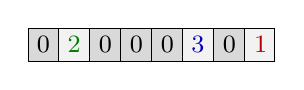
\begin{tikzpicture}[
    mpnv/.style = {rectangle split, rectangle split horizontal,
      rectangle split parts=8,
      rectangle split part fill={gray!30,gray!10,gray!30,gray!30,gray!30,
                                gray!10,gray!30,gray!10},
      draw, text width=0.5em, align=center, minimum height=1em},
  ]
\node[mpnv] (C)
    {\nodepart{one}     0
     \nodepart{two}     \textcolor{mygreen}{2}
     \nodepart{three}   0
     \nodepart{four}    0
     \nodepart{five}    0
     \nodepart{six}     \textcolor{myblue}{3}
     \nodepart{seven}   0
     \nodepart{eight}   \textcolor{myred}{1}
    };
\draw (C) -- (C);
\end{tikzpicture}
\end{column}
\begin{column}{.60\linewidth}
$\var{cost} = \frac{1}{\textcolor{mygreen}{2} + \textcolor{myblue}{3} + \textcolor{myred}{1}} \big(\textcolor{mygreen}{2}\frac{1+\textcolor{mygreen}{2}}{2} + \textcolor{myblue}{3}\frac{1+\textcolor{myblue}{3}}{2} + \textcolor{myred}{1}\frac{1+\textcolor{myred}{1}}{2}\big) \approx 1.66$
\end{column}
\end{columns}
\pause

A \emph{perfect hash} fills buckets as evenly as possible.\\
They have minimal cost:
\vspace{0.2\baselineskip}
\begin{columns}
\begin{column}{.40\linewidth}
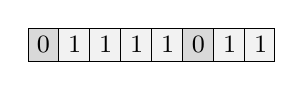
\begin{tikzpicture}[
    mpnv/.style = {rectangle split, rectangle split horizontal,
      rectangle split parts=8,
      rectangle split part fill={gray!30,gray!10,gray!10,gray!10,gray!10,
                                gray!30,gray!10,gray!10},
      draw, text width=0.5em, align=center, minimum height=1em},
  ]
\node[mpnv] (C)
    {\nodepart{one}     0
     \nodepart{two}     1
     \nodepart{three}   1
     \nodepart{four}    1
     \nodepart{five}    1
     \nodepart{six}     0
     \nodepart{seven}   1
     \nodepart{eight}   1
    };
\draw (C) -- (C);
\end{tikzpicture}
\end{column}
\begin{column}{.60\linewidth}
$\var{cost} = 1$
\end{column}
\end{columns}
\pause
The \emph{regret} is the cost minus the minimum achievable cost.

\pause
A \emph{uniform hash} assigns each key to a bucket with the same probability.\\
0.5 expected regret at load factor 1 (eaten by $\mathcal{O()}$).

\mglconclusion{There is something to gain even in theory.}
\end{frame}

\begin{frame}
\frametitle{\textcolor{black}{\Motivation:} Setup for the Reality Check}
The theoretical cost model is bad (duh).

Case-study on Integer Hashing:
\begin{itemize}
\item Keys: machine words (e.g. integer, pointer)
\item Implementation: Common Lisp (SBCL)
\item Comparison function: \lisp{eq} (like \inlinett{==} in Java or \inlinett{CMP} in assembly)
\item Hash function: integer value / address $\rightarrow$ hash value
\end{itemize}

We compare
\begin{itemize}
\item \textcolor{murmurhashcolor}{Murmur}3 mixer: a general-purpose hash function ($\sim$ Uniform Hash)
\item \textcolor{prefuzzhashcolor}{Prefuzz}: SBCL's own hand-crafted \lisp{eq} hash.
\end{itemize}
\end{frame}

\begin{frame}
\frametitle{\textcolor{black}{\Motivation:} Hash Function Speed Matters}
\begin{columns}
\begin{column}{.40\linewidth}
\lisp{Eq} hash table performance vs the number of keys with \textcolor{murmurhashcolor}{Murmur} and \textcolor{prefuzzhashcolor}{Prefuzz}.

\textbf{Keys}: random existing symbol objects

\textbf{Regret}: Sameish. Close to a Uniform Hash.

\textbf{Put, Get}: Prefuzz is 5--15\% faster (to compute).
\end{column}
\begin{column}{.60\linewidth}
\figurecolumn
\begin{figure}[H]
\begin{tikzpicture}
  \begin{axis}[xlabel=\textbf{\scriptsize \#keys}, ylabel=\textbf{regret},
      x label style={at={(ticklabel* cs:1.03)},anchor=north east},
      xmin=1, xmode=log, log basis x={2},
      ymin=-0.01, ymax=0.79,
      legend pos=north west,
      legend columns=2,
      legend style={nodes={scale=0.7, transform shape}},
      legend cell align={left},
      height=0.55\linewidth,
      width=0.98\linewidth,
    ]
    \pgfplotstableread{../paper/data/symbol-existing-murmur.tbl}{\sorted}
    \addplot[murmurhash] table [x=nkeys, y=regret] {\sorted};

    \pgfplotstableread{../paper/data/symbol-existing-prefuzz.tbl}{\sorted}
    \addplot[prefuzzhash] table [x=nkeys, y=regret] {\sorted};
  \end{axis}
\end{tikzpicture}
\end{figure}
\begin{figure}[H]
\begin{tikzpicture}
  \begin{axis}[ylabel=ns / \textbf{put},
      xmin=1, xmode=log, log basis x={2},
      ymin=20, ymax=180, ymode=log, log basis y={2},
      legend pos=north west,
      legend style={nodes={scale=0.7, transform shape}},
      legend cell align={left},
      height=0.55\linewidth,
      width=0.98\linewidth,
    ]
    \pgfplotstableread{../paper/data/symbol-existing-murmur.tbl}{\sorted}
    \addplot[murmurhash] table [x=nkeys, y=putns] {\sorted};

    \pgfplotstableread{../paper/data/symbol-existing-prefuzz.tbl}{\sorted}
    \addplot[prefuzzhash] table [x=nkeys, y=putns] {\sorted};
  \end{axis}
\end{tikzpicture}
\end{figure}

\begin{figure}[H]
\begin{tikzpicture}
  \begin{axis}[ylabel=ns / \textbf{get},
      xmin=1, xmode=log, log basis x={2},
      ymin=6, ymax=180, ymode=log, log basis y={2},
      legend pos=north west,
      legend style={nodes={scale=0.7, transform shape}},
      legend cell align={left},
      height=0.55\linewidth,
      width=0.98\linewidth,
    ]
    \pgfplotstableread{../paper/data/symbol-existing-murmur.tbl}{\sorted}
    \addplot[murmurhash] table [x=nkeys, y=getns] {\sorted};

    \pgfplotstableread{../paper/data/symbol-existing-prefuzz.tbl}{\sorted}
    \addplot[prefuzzhash] table [x=nkeys, y=getns] {\sorted};
  \end{axis}
\end{tikzpicture}
\end{figure}
\end{column}
\end{columns}
\end{frame}

\begin{frame}
\frametitle{\textcolor{black}{\Motivation:} Cache-friendliness Matters}
\begin{columns}
\begin{column}{.40\linewidth}
\textbf{Keys}: integer arithmetic progressions with increment 1 (e.g. 1, 2, 3, $\dots$).

\textbf{Regret}: Is \textcolor{prefuzzhashcolor}{Prefuzz} optimized for small hash tables?

\textbf{Put}: Prefuzz is 20--75\% faster due to local collisions.

\textbf{Get}: Randomized query order $\Rightarrow$ smaller gains
\end{column}
\begin{column}{.60\linewidth}
\figurecolumn
\begin{figure}[H]
\begin{tikzpicture}
  \begin{axis}[ylabel=regret,
      xmin=1, xmode=log, log basis x={2},
      ymin=-0.01, ymax=0.79,
      legend pos=north west,
      legend columns=2,
      legend style={nodes={scale=0.7, transform shape}},
      legend cell align={left},
      height=0.55\linewidth,
      width=0.98\linewidth,
    ]
    \pgfplotstableread{../paper/data/fixnum-prog-1-murmur.tbl}{\sorted}
    \addplot[murmurhash] table [x=nkeys, y=regret] {\sorted};

    \pgfplotstableread{../paper/data/fixnum-prog-1-prefuzz.tbl}{\sorted}
    \addplot[prefuzzhash] table [x=nkeys, y=regret] {\sorted};
  \end{axis}
\end{tikzpicture}
\end{figure}

\begin{figure}[H]
\begin{tikzpicture}
  \begin{axis}[ylabel=ns / put,
      xmin=1, xmode=log, log basis x={2},
      ymin=20, ymax=180, ymode=log, log basis y={2},
      legend pos=north west,
      legend style={nodes={scale=0.7, transform shape}},
      legend cell align={left},
      height=0.55\linewidth,
      width=0.98\linewidth,
    ]
    \pgfplotstableread{../paper/data/fixnum-prog-1-murmur.tbl}{\sorted}
    \addplot[murmurhash] table [x=nkeys, y=putns] {\sorted};

    \pgfplotstableread{../paper/data/fixnum-prog-1-prefuzz.tbl}{\sorted}
    \addplot[prefuzzhash] table [x=nkeys, y=putns] {\sorted};
  \end{axis}
\end{tikzpicture}
\end{figure}

\begin{figure}[H]
\begin{tikzpicture}
  \begin{axis}[ylabel=ns / get,
      xmin=1, xmode=log, log basis x={2},
      ymin=6, ymax=180, ymode=log, log basis y={2},
      legend pos=north west,
      legend style={nodes={scale=0.7, transform shape}},
      legend cell align={left},
      height=0.55\linewidth,
      width=0.98\linewidth,
    ]
    \pgfplotstableread{../paper/data/fixnum-prog-1-murmur.tbl}{\sorted}
    \addplot[murmurhash] table [x=nkeys, y=getns] {\sorted};

    \pgfplotstableread{../paper/data/fixnum-prog-1-prefuzz.tbl}{\sorted}
    \addplot[prefuzzhash] table [x=nkeys, y=getns] {\sorted};
  \end{axis}
\end{tikzpicture}
\end{figure}
\end{column}
\end{columns}
\end{frame}

\begin{frame}
\frametitle{\textcolor{black}{\Motivation:} Not Crashing and Burning Matters}
\begin{columns}
\begin{column}{.40\linewidth}
\textbf{Keys}: single float arithmetic progressions (e.g. 1.0, 2.0, 3.0, $\dots$)

\textcolor{prefuzzhashcolor}{Prefuzz} breaks.
\end{column}
\begin{column}{.60\linewidth}
\figurecolumn
\begin{figure}[H]
\begin{tikzpicture}
  \begin{axis}[ylabel=regret \textbf{(log)},
      xmin=1, xmode=log, log basis x={2},
      ymin=0.1, ymax=2000, ymode=log, log basis y={10},
      ytick={1, 100},
      %% extra y ticks={
      %%   0.001, 0.0028, 0.0046, 0.0064, 0.0082,
      %%   0.1, 0.28, 0.46, 0.64, 0.82,
      %%   10, 28, 46, 64, 82,
      %%   1000, 2800, 4600, 6400, 8200},
      %% extra y tick labels={},
      legend pos=south east,
      legend columns=2,
      legend style={nodes={scale=0.7, transform shape}},
      legend cell align={left},
      height=0.55\columnwidth,
      width=0.98\columnwidth,
    ]
    \pgfplotstableread{../paper/data/float-prog-1-murmur.tbl}{\sorted}
    \addplot[murmurhash] table [x=nkeys, y=regret] {\sorted};

    \pgfplotstableread{../paper/data/float-prog-1-prefuzz.tbl}{\sorted}
    \addplot[prefuzzhash] table [x=nkeys, y expr={min(\thisrow{regret}, 2000)}] {\sorted};
  \end{axis}
\end{tikzpicture}
\end{figure}
\begin{figure}[H]
\begin{tikzpicture}
  \begin{axis}[ylabel=ns / put,
      xmin=1, xmode=log, log basis x={2},
      ymin=20, ymax=2000, ymode=log, log basis y={2},
      legend pos=north east,
      legend style={nodes={scale=0.7, transform shape}},
      legend cell align={left},
      height=0.55\columnwidth,
      width=0.98\columnwidth,
    ]
    \pgfplotstableread{../paper/data/float-prog-1-murmur.tbl}{\sorted}
    \addplot[murmurhash] table [x=nkeys, y=putns] {\sorted};

    \pgfplotstableread{../paper/data/float-prog-1-prefuzz.tbl}{\sorted}
    \addplot[prefuzzhash] table [x=nkeys, y=putns] {\sorted};
  \end{axis}
\end{tikzpicture}
\end{figure}
\begin{figure}[H]
\begin{tikzpicture}
  \begin{axis}[ylabel=ns / get,
      xmin=1, xmode=log, log basis x={2},
      ymin=6, ymax=2000, ymode=log, log basis y={2},
      legend pos=north east,
      legend style={nodes={scale=0.7, transform shape}},
      legend cell align={left},
      height=0.55\columnwidth,
      width=0.98\columnwidth,
    ]
    \pgfplotstableread{../paper/data/float-prog-1-murmur.tbl}{\sorted}
    \addplot[murmurhash] table [x=nkeys, y=getns] {\sorted};

    \pgfplotstableread{../paper/data/float-prog-1-prefuzz.tbl}{\sorted}
    \addplot[prefuzzhash] table [x=nkeys, y=getns] {\sorted};
  \end{axis}
\end{tikzpicture}
\end{figure}
\end{column}
\end{columns}
\end{frame}

\begin{frame}
\frametitle{\textcolor{black}{\Motivation:} A Compromise W\hspace{-0.09em}aiting to Happen}
General-purpose hash functions (e.g. Murmur):
\begin{itemize}
\item \emph{robust} (work with any key distribution)
\item \emph{wasteful} (do computation that doesn't improve performance)
\item \emph{suboptimal} (non-zero regret, about 0.5)
\item \emph{cache-unfriendly}
\end{itemize}

Hand-crafted hash functions (e.g. Prefuzz) are the opposite:
\begin{itemize}
\item \emph{fragile} (fail outside the intended key distribution)
\item \emph{frugal} (perform minimal computation)
\item can be \emph{optimal} (zero regret)
\item can be \emph{cache-friendly}
\end{itemize}
\end{frame}


\begin{frame}
\frametitle{\Adaptive{} \Hashing}
% Overlay and tikzexternalize conflict
\tikzset{external/export next=false}
\begin{tikzpicture}[overlay, remember picture]
\node[] at (current page.north east) [anchor = north east,
  xshift=-0.8cm, yshift=-0.7cm]
{
    \rotatebox{-60}{%
      \href{https://www.theguardian.com/lifeandstyle/wordofmouth/2012/oct/18/how-to-cook-perfect-hash-browns}%
           {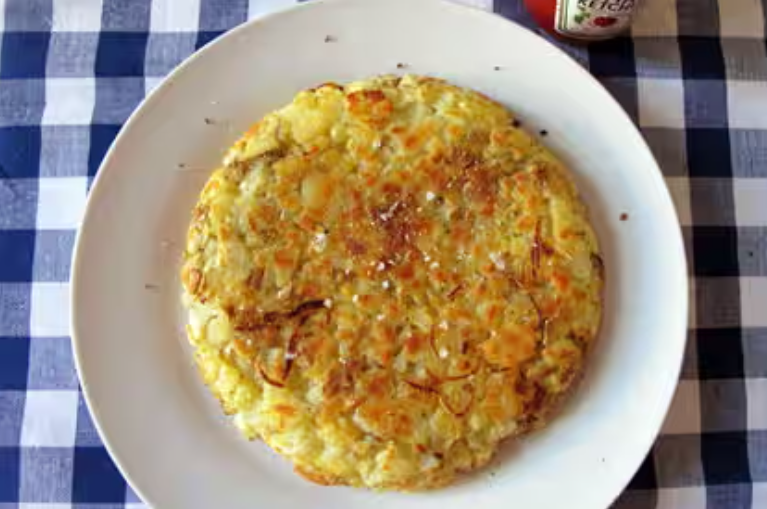
\includegraphics[width=0.3\textwidth]{perfect-hash-brown.png}}}
};
\end{tikzpicture}
Won't do:
\begin{itemize}
\item Perfect Hashing: static key set, offline, slow
\item Dynamic Perfect Hashing: much more memory
\end{itemize}

Will do:
\begin{itemize}
\item Adapt the hash function to the current set of keys
\item online
\item to be faster
\item with no change to the hash table API.
\end{itemize}
Can do fast enough?
\end{frame}

\begin{frame}
\frametitle{\textcolor{black}{\Adaptive{} \Hashing:} Skeleton}
\begin{columns}
\begin{column}{.45\linewidth}
Three low-overhead triggers for adaptation in $\fn{put}()$:
\begin{itemize}
\item Max chain length
\item Collision count at rehash
\item Hash table size
\end{itemize}
\end{column}
\begin{column}{.55\linewidth}
  \begin{algorithmic}[0]
    \color{gray!100}
    \Function{$\fn{put}$}{$\var{key}$, $\var{value}$}
      \Let{$\var{bucket}$}{$h(\var{key}) \bmod m$}
      \color{mglred2}
      \Let{$\var{chain\_length}$}{$0$}
      \color{gray!100}
      \For{$k$ $\gets$ next key in $\var{bucket}$}
        \If{$\fn{compare}(\var{key}, k)$}
          \Let{value of $k$}{$\var{value}$}
          \State\Return
        \EndIf
        \color{mglred2}
        \Let{$\var{chain\_length}$}{$\var{chain\_length} + 1$}
        \color{gray!100}
      \EndFor
      \pause
      \color{mglred2}
      \If{$\var{chain\_length}$ too high}
        \Let{$h$}{$\fn{safer\_hash\_function}(h)$}
        \Let{$\var{bucket}$}{$h(\var{key}) \bmod m$}
      \EndIf
      \color{gray!100}
      \pause
      \If{hash table is full}
        \State{double $m$ and increase storage}
        \color{mglred2}
        \Let{$h$}{$\textcolor{gray}{%
            \fn{\textcolor{mglred2}{adapt\_and\_}rehash}(h, m)}$}
        \If{$h$ was changed}
          \Let{$\var{bucket}$}{$h(\var{key}) \bmod m$}
        \EndIf
        \color{gray!100}
      \EndIf
      \State{add $(\var{key}, \var{value})$ to $\var{bucket}$}
    \EndFunction
  \end{algorithmic}
\end{column}
\end{columns}
\end{frame}


\begin{frame}
\frametitle{\Adaptive{} Eq}
More concretely, for \lisp{Eq} hashing:
{
\setlength{\parskip}{0pt}
\begin{enumerate}
\item Init to \emph{Constant hash}: linear search in a vector internally \lispersonly{(no extra overhead for keys moved by GC)}
\item $\rightarrow$ \emph{Pointer-Shift} above 32 keys
\item $\rightarrow$ \emph{Prefuzz} if doing badly
\item $\rightarrow$ \emph{Murmur} similarly
\end{enumerate}
\vspace{-4\baselineskip}
\hspace{15em}\scalebox{0.6}{\rotatebox{55}{\href{%
      https://en.wikipedia.org/wiki/Jenkins_hash_function}%
    {\includesvg{JenkinsOneAtATime-3.svg}}}}%
\vspace{-5\baselineskip}
}
%% Separate hash table accessors for Constant and Murmur.
%%
%% Regret would be better, but even collision counting has overhead.
\end{frame}

\begin{frame}[fragile]
\frametitle{\textcolor{black}{\Adaptive{} Eq:} Page-based Memory Allocation}
Memory addresses of objects are unique.

Allocators grab a contiguous memory range from the OS (expensive).

Then, they cram many small objects into these ``pages''.

Most allocations are just a pointer bump (cheap).

\mglconclusion{Addresses resemble arithmetic progressions within pages.}
\end{frame}

\begin{frame}[fragile]
\frametitle{\textcolor{black}{\Adaptive{} Eq:} The Arithmetic Hash}
Arithmetic progressions with odd increments are perfect hashes in power-of-2 hash tables (coprimes).

Let $s$ be the number of low bits which are the same in all keys.

\mglconclusion{$k \rightarrow k \gg s$ is a \emph{perfect hash} for all arithmetic progressions.}
%% Example:
%% \begin{align*}
%% 28 \rightarrow \phantom{0}7 \bmod 4 = 3 \\
%% 56 \rightarrow 14 \bmod 4 = 2 \\
%% 84 \rightarrow 21 \bmod 4 = 1 \\
%% 56 \rightarrow 28 \bmod 4 = 0
%% \end{align*}
\pause
\\[2\baselineskip]
Computing $s$ is cheap:
\\[2\baselineskip]
\begin{algorithmic}[0]
  \Function{$\fn{count\_common\_prefix\_bits}$}{$k_1, \dots, k_n$}
  \Let{$\var{mask}$}{$0$}
  \Comment{Changed bits detected so far}
  \For{$i \gets 2$ to $n$}
  \State{$\var{mask} \gets \var{mask} \lor (k_1 \oplus k_i)$}
  \Comment{One \texttt{OR} and one \texttt{XOR} instruction}
  \EndFor
  \State\Return{$\fn{count\_leading\_zero\_bits}(\lnot \var{mask})$}
  \Comment{A single \texttt{LZCNT} instruction}
  \EndFunction
\end{algorithmic}
\end{frame}

\begin{frame}[fragile]
\frametitle{\textcolor{black}{\Adaptive{} Eq:} The Pointer-Mix Hash}
Multiple pages: less regular allocation patterns

Keep the low bits intact, and \textcolor{mglred2}{mix in the page}:
\begin{align*}
\fn{pointer\_mix}(k) = k \gg s \hspace{0.5ex} \textcolor{mglred2}{\oplus \fn{uniform\_hash}(k \gg \var{n\_page\_bits})}
\end{align*}

For random subsets of arithmetic progressions, Pointer-Mix
\begin{itemize}
\item is a Perfect Hash with all keys on a single page;
\item behaves like a Uniform Hash with more pages.
\end{itemize}
\end{frame}

\begin{frame}[fragile]
\frametitle{\textcolor{black}{\Adaptive{} Eq:} The Pointer-Shift Hash}
Pointer-Mix is easy to analyse but slow due to $\fn{uniform\_hash}()$.

Mix in the page faster $\rightarrow$ Pointer-Shift:
{
\begin{verbatim}
  address >> s +           /* Remove the constant low bits */
  address >> n_page_bits   /* Mix in page address          */
\end{verbatim}
}
Extremely aggressive, but it has Prefuzz as a safety net.
\end{frame}

\begin{frame}[fragile]
\frametitle{\textcolor{black}{\Adaptive{} Eq:} The Prefuzz Hash}
Stock SBCL's \lisp{eq} hash is Prefuzz:

{
\begin{verbatim}
  address ^ 0xdeadbeef +  /* Destroy some regular patterns */
  address >> 1 +          /* Mix the low bits a bit        */
  address >> 4 +
  address >> 13 +
  address >> 21           /* Ignore the high bits          */
\end{verbatim}
}
So that's why it worked well until it didn't: it punts on the high bits.

Plays it safer than Adaptive but still needs Murmur as a safety net.

\mglconclusion{Similar to Pointer-Shift but does not depend on the other keys!}
\end{frame}

\begin{frame}<0>
\frametitle{\Adaptive{} Eq}
\begin{columns}
\begin{column}{.36\linewidth}
The constant hash is really a specialized implementation with a vector and linear search. No need to track objects moved by the GC.


\end{column}
\begin{column}{.64\linewidth}
  \begin{algorithmic}[0]\footnotesize
    \Require{Integer/pointer keys $k_{i:n}$, doubled number of buckets $m$, current hash function $h$.}
    \Procedure{$\fn{adapt\_and\_rehash\_eq}$}{}
      \If{h = constant\_hash}
        \If{m = 64}
          \Let{$s$}{
            $\fn{count\_common\_prefix\_bits}(\textrm{k}_{1:10}$)}
          \Let{$h$}{$\fn{pointer\_shift}$}
        \EndIf
      \EndIf
      \If{$h = \fn{pointer\_shift}$}
        \Let{$\var{n\_collisions}$}{
          $\fn{rehash\_and\_count}(m, h)$}
        \If{$\var{n\_collisions}$ is too many}
          \Let{$h$}{$\fn{prefuzz}$}
        \EndIf
      \EndIf
      \If{$h = \fn{prefuzz}$}
        \If{$m < 2048$}
          \State{$\fn{rehash}(m, h)$}
        \Else
          \Let{$\var{n\_collisions}$}{
            $\fn{rehash\_and\_count}(m, h)$}
          \If{$\var{n\_collisions}$ is too many}
            \Let{$h$}{$\fn{murmur3}$}
          \EndIf
        \EndIf
      \EndIf
      \If{$h = \fn{murmur3}$}
        \State $\fn{rehash}(m, h)$
      \EndIf
    \EndProcedure
  \end{algorithmic}
\end{column}
\end{columns}
\end{frame}

\begin{frame}
\frametitle{\textcolor{black}{\Adaptive{} Eq:} Faster \Hashing}
\begin{columns}
\begin{column}{.40\linewidth}
\textbf{Keys}: random existing symbol objects (revisited)

\textbf{Regret}: Sameish. Not plotting the Constant phase.

\textbf{Put}: Big win for \textcolor{adaptivehashcolor}{Adaptive} in the Constant phase.

\textbf{Get}: A few percent faster than \textcolor{prefuzzhashcolor}{Prefuzz}, which is already better than \textcolor{murmurhashcolor}{Murmur} due to being a faster hash function.
\end{column}
\begin{column}{.60\linewidth}
\figurecolumn
\begin{figure}[H]
\begin{tikzpicture}
  \begin{axis}[ylabel=regret,
      xmin=1, xmode=log, log basis x={2},
      ymin=-0.01, ymax=0.79,
      legend pos=north west,
      legend columns=2,
      legend style={nodes={scale=0.7, transform shape}},
      legend cell align={left},
      height=0.55\linewidth,
      width=0.98\linewidth,
    ]
    \pgfplotstableread{../paper/data/symbol-existing-murmur.tbl}{\sorted}
    \addplot[murmurhash] table [x=nkeys, y=regret] {\sorted};

    \pgfplotstableread{../paper/data/symbol-existing-prefuzz.tbl}{\sorted}
    \addplot[prefuzzhash] table [x=nkeys, y=regret] {\sorted};

    \pgfplotstableread{../paper/data/symbol-existing-flat-safe-small.tbl}
                      {\sorted}
    \addplot[adaptivehash] table [x=nkeys, y=regret] {\sorted};
  \end{axis}
\end{tikzpicture}
\end{figure}

\begin{figure}[H]
\begin{tikzpicture}
  \begin{axis}[ylabel=ns / put,
      xmin=1, xmode=log, log basis x={2},
      ymin=20, ymax=180, ymode=log, log basis y={2},
      legend pos=north west,
      legend style={nodes={scale=0.7, transform shape}},
      legend cell align={left},
      height=0.55\linewidth,
      width=0.98\linewidth,
    ]
    \pgfplotstableread{../paper/data/symbol-existing-murmur.tbl}{\sorted}
    \addplot[murmurhash] table [x=nkeys, y=putns] {\sorted};

    \pgfplotstableread{../paper/data/symbol-existing-prefuzz.tbl}{\sorted}
    \addplot[prefuzzhash] table [x=nkeys, y=putns] {\sorted};

    \pgfplotstableread{../paper/data/symbol-existing-flat-safe-small.tbl}
                      {\sorted}
    \addplot[adaptivehash] table [x=nkeys, y=putns] {\sorted};
  \end{axis}
\end{tikzpicture}
\end{figure}

\begin{figure}[H]
\begin{tikzpicture}
  \begin{axis}[ylabel=ns / get,
      xmin=1, xmode=log, log basis x={2},
      ymin=6, ymax=180, ymode=log, log basis y={2},
      legend pos=north west,
      legend style={nodes={scale=0.7, transform shape}},
      legend cell align={left},
      height=0.55\linewidth,
      width=0.98\linewidth,
    ]
    \pgfplotstableread{../paper/data/symbol-existing-murmur.tbl}{\sorted}
    \addplot[murmurhash] table [x=nkeys, y=getns] {\sorted};

    \pgfplotstableread{../paper/data/symbol-existing-prefuzz.tbl}{\sorted}
    \addplot[prefuzzhash] table [x=nkeys, y=getns] {\sorted};

    \pgfplotstableread{../paper/data/symbol-existing-flat-safe-small.tbl}
                      {\sorted}
    \addplot[adaptivehash] table [x=nkeys, y=getns] {\sorted};
  \end{axis}
\end{tikzpicture}
\end{figure}
\end{column}
\end{columns}
\end{frame}

\begin{frame}
\frametitle{\textcolor{black}{\Adaptive{} Eq:} Less Regret}
\begin{columns}
\begin{column}{.40\linewidth}
\textbf{Keys}: integer arithmetic progression (revisited)

\textbf{Regret}: \textcolor{adaptivehashcolor}{Adaptive} is a perfect hash.

\textbf{Put}: 50\% over \textcolor{murmurhashcolor}{Murmur}, and over \textcolor{prefuzzhashcolor}{Prefuzz} in the Constant hash phase

\textbf{Get}: Up to 50\% faster
\end{column}
\begin{column}{.60\linewidth}
\figurecolumn
\begin{figure}[H]
\begin{tikzpicture}
  \begin{axis}[ylabel=regret,
      xmin=1, xmode=log, log basis x={2},
      ymin=-0.01, ymax=0.79,
      legend pos=north west,
      legend columns=2,
      legend style={nodes={scale=0.7, transform shape}},
      legend cell align={left},
      height=0.55\linewidth,
      width=0.98\linewidth,
    ]
    \pgfplotstableread{../paper/data/fixnum-prog-1-murmur.tbl}{\sorted}
    \addplot[murmurhash] table [x=nkeys, y=regret] {\sorted};

    \pgfplotstableread{../paper/data/fixnum-prog-1-prefuzz.tbl}{\sorted}
    \addplot[prefuzzhash] table [x=nkeys, y=regret] {\sorted};

    \pgfplotstableread{../paper/data/fixnum-prog-1-flat-safe-small.tbl}{\sorted}
    \addplot[adaptivehash] table [x=nkeys, y=regret] {\sorted};
  \end{axis}
\end{tikzpicture}
\end{figure}

\begin{figure}[H]
\begin{tikzpicture}
  \begin{axis}[ylabel=ns / put,
      xmin=1, xmode=log, log basis x={2},
      ymin=20, ymax=180, ymode=log, log basis y={2},
      legend pos=north west,
      legend style={nodes={scale=0.7, transform shape}},
      legend cell align={left},
      height=0.55\linewidth,
      width=0.98\linewidth,
    ]
    \pgfplotstableread{../paper/data/fixnum-prog-1-murmur.tbl}{\sorted}
    \addplot[murmurhash] table [x=nkeys, y=putns] {\sorted};

    \pgfplotstableread{../paper/data/fixnum-prog-1-prefuzz.tbl}{\sorted}
    \addplot[prefuzzhash] table [x=nkeys, y=putns] {\sorted};

    \pgfplotstableread{../paper/data/fixnum-prog-1-flat-safe-small.tbl}{\sorted}
    \addplot[adaptivehash] table [x=nkeys, y=putns] {\sorted};
  \end{axis}
\end{tikzpicture}
\end{figure}

\begin{figure}[H]
\begin{tikzpicture}
  \begin{axis}[ylabel=ns / get,
      xmin=1, xmode=log, log basis x={2},
      ymin=6, ymax=180, ymode=log, log basis y={2},
      legend pos=north west,
      legend style={nodes={scale=0.7, transform shape}},
      legend cell align={left},
      height=0.55\linewidth,
      width=0.98\linewidth,
    ]
    \pgfplotstableread{../paper/data/fixnum-prog-1-murmur.tbl}{\sorted}
    \addplot[murmurhash] table [x=nkeys, y=getns] {\sorted};

    \pgfplotstableread{../paper/data/fixnum-prog-1-prefuzz.tbl}{\sorted}
    \addplot[prefuzzhash] table [x=nkeys, y=getns] {\sorted};

    \pgfplotstableread{../paper/data/fixnum-prog-1-flat-safe-small.tbl}{\sorted}
    \addplot[adaptivehash] table [x=nkeys, y=getns] {\sorted};
  \end{axis}
\end{tikzpicture}
\end{figure}
\end{column}
\end{columns}
\end{frame}

\begin{frame}
\frametitle{\textcolor{black}{\Adaptive{} Eq:} More Robustness}
\begin{columns}
\begin{column}{.40\linewidth}
\textbf{Keys}: single float arithmetic progressions (revisited)

\textcolor{adaptivehashcolor}{Adaptive} takes advantage of the regularity.
When its guessed shift becomes incorrect, it falls back to \textcolor{prefuzzhashcolor}{Prefuzz} (a bad idea) and then immediately to \textcolor{murmurhashcolor}{Murmur}.
\end{column}
\begin{column}{.60\linewidth}
\figurecolumn
\begin{figure}[H]
\begin{tikzpicture}
  \begin{axis}[ylabel=regret \textbf{(log)},
      xmin=1, xmode=log, log basis x={2},
      ymin=0.001, ymax=2000, ymode=log, log basis y={10},
      ytick={0.01, 1, 100},
      yticklabels={$10^{\shortminus 2}$, $10^0$, $10^2$},
      %% extra y ticks={
      %%   0.001, 0.0028, 0.0046, 0.0064, 0.0082,
      %%   0.1, 0.28, 0.46, 0.64, 0.82,
      %%   10, 28, 46, 64, 82,
      %%   1000, 2800, 4600, 6400, 8200},
      %% extra y tick labels={},
      legend pos=south east,
      legend columns=2,
      legend style={nodes={scale=0.7, transform shape}},
      legend cell align={left},
      height=0.55\columnwidth,
      width=0.98\columnwidth,
    ]
    \pgfplotstableread{../paper/data/float-prog-1-murmur.tbl}{\sorted}
    \addplot[murmurhash] table [x=nkeys, y=regret] {\sorted};

    \pgfplotstableread{../paper/data/float-prog-1-prefuzz.tbl}{\sorted}
    \addplot[prefuzzhash] table [x=nkeys, y expr={min(\thisrow{regret}, 2000)}] {\sorted};

    \pgfplotstableread{../paper/data/float-prog-1-flat-safe-small.tbl}{\sorted}
    \addplot[adaptivehash] table [x=nkeys, y expr={min(\thisrow{regret}, 2000)}] {\sorted};
  \end{axis}
\end{tikzpicture}
\end{figure}
\begin{figure}[H]
\begin{tikzpicture}
  \begin{axis}[ylabel=ns / put,
      xmin=1, xmode=log, log basis x={2},
      ymin=20, ymax=200, ymode=log, log basis y={2},
      legend pos=north east,
      legend style={nodes={scale=0.7, transform shape}},
      legend cell align={left},
      height=0.55\columnwidth,
      width=0.98\columnwidth,
    ]
    \pgfplotstableread{../paper/data/float-prog-1-murmur.tbl}{\sorted}
    \addplot[murmurhash] table [x=nkeys, y=putns] {\sorted};

    \pgfplotstableread{../paper/data/float-prog-1-prefuzz.tbl}{\sorted}
    \addplot[prefuzzhash] table [x=nkeys, y=putns] {\sorted};

    \pgfplotstableread{../paper/data/float-prog-1-flat-safe-small.tbl}{\sorted}
    \addplot[adaptivehash] table [x=nkeys, y=putns] {\sorted};
  \end{axis}
\end{tikzpicture}
\end{figure}
\begin{figure}[H]
\begin{tikzpicture}
  \begin{axis}[ylabel=ns / get,
      xmin=1, xmode=log, log basis x={2},
      ymin=6, ymax=200, ymode=log, log basis y={2},
      legend pos=north east,
      legend style={nodes={scale=0.7, transform shape}},
      legend cell align={left},
      height=0.55\columnwidth,
      width=0.98\columnwidth,
    ]
    \pgfplotstableread{../paper/data/float-prog-1-murmur.tbl}{\sorted}
    \addplot[murmurhash] table [x=nkeys, y=getns] {\sorted};

    \pgfplotstableread{../paper/data/float-prog-1-prefuzz.tbl}{\sorted}
    \addplot[prefuzzhash] table [x=nkeys, y=getns] {\sorted};

    \pgfplotstableread{../paper/data/float-prog-1-flat-safe-small.tbl}{\sorted}
    \addplot[adaptivehash] table [x=nkeys, y=getns] {\sorted};
  \end{axis}
\end{tikzpicture}
\end{figure}
\end{column}
\end{columns}
\end{frame}

\begin{frame}[fragile]
\frametitle{\textcolor{black}{\Adaptive{} Eq:} Made in Heaven}
\vspace{0.5\baselineskip}
\begin{center}
\scalebox{0.4}{
\fontsize{10.290958pt}{16pt}
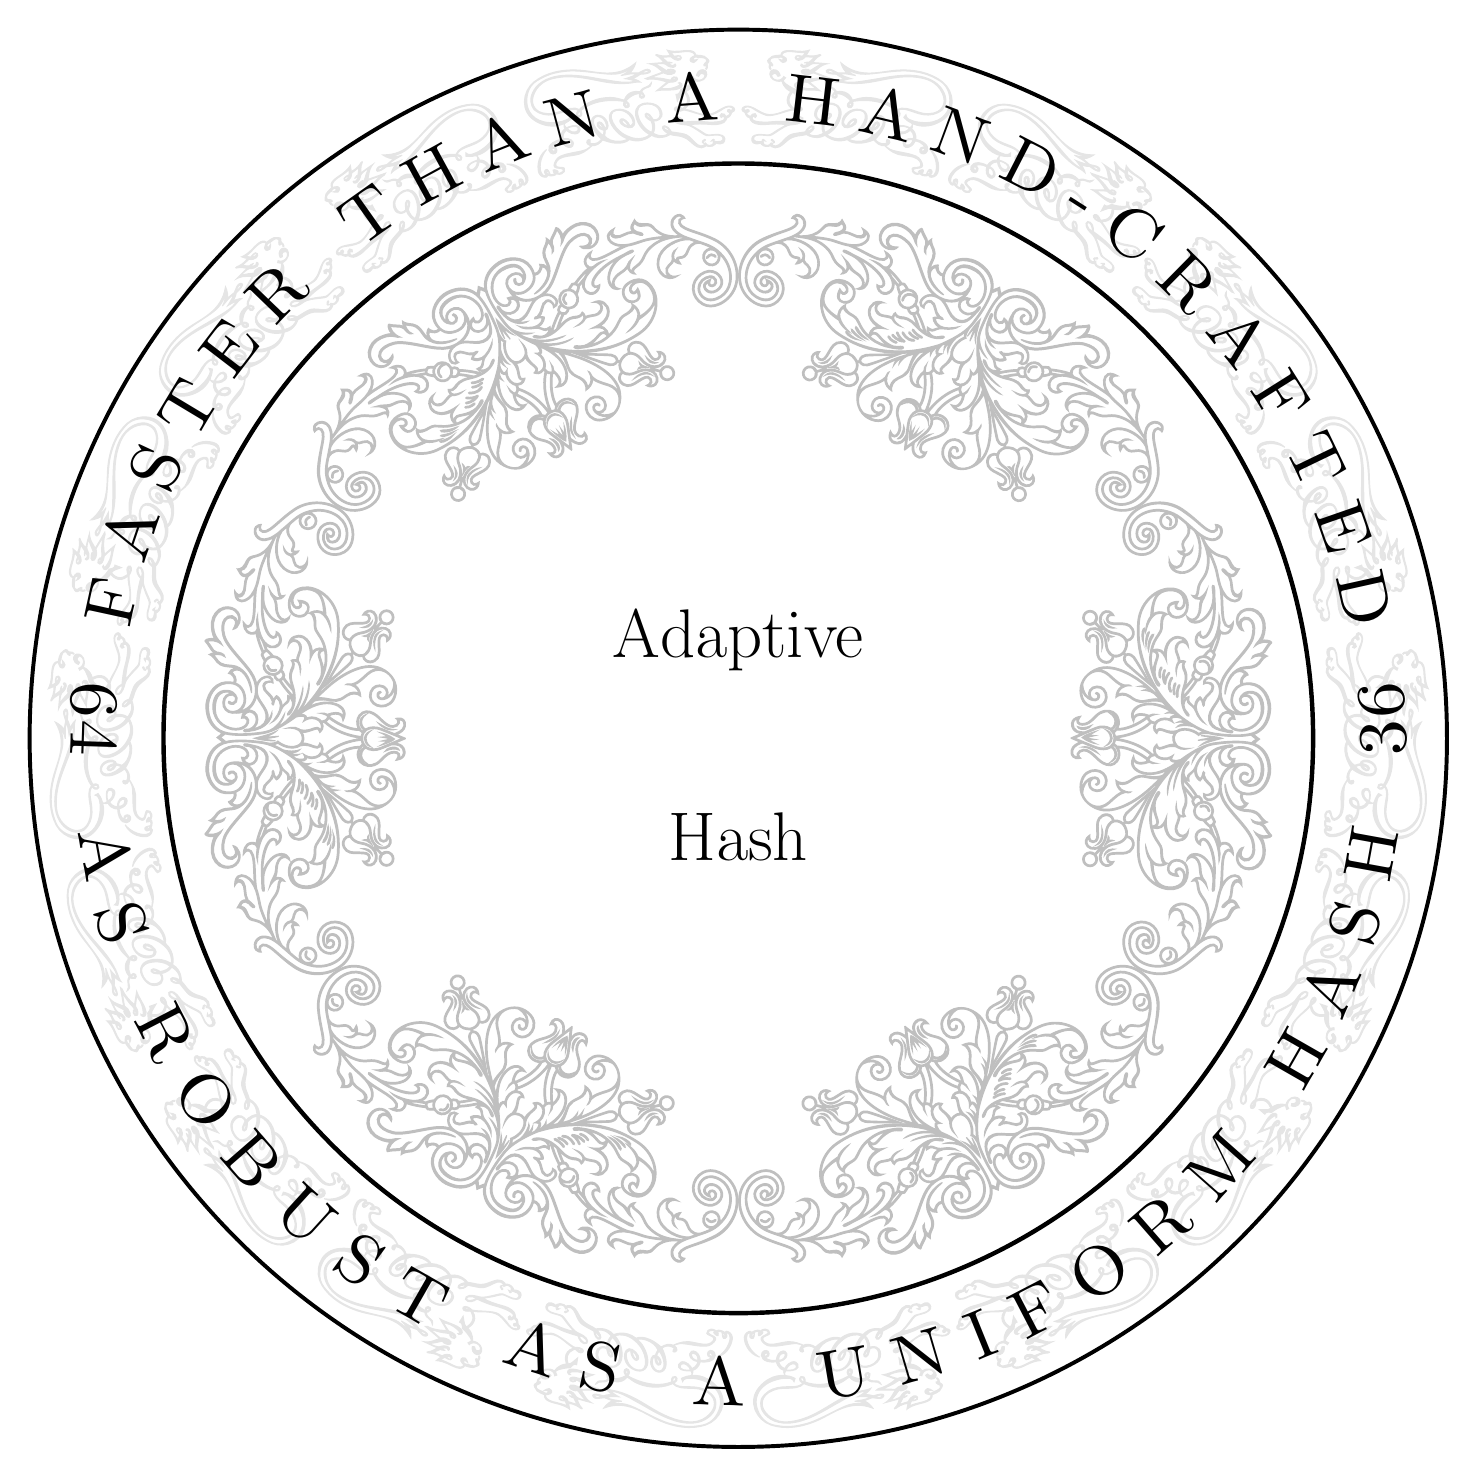
\begin{tikzpicture}
  %%%% Text along circular path
  % outer circle
  \draw[line width=0.5 mm] circle[radius=9 cm];
  % inner circles
  \draw[ultra thick]  circle[radius=7.3 cm];
  % Chain of lions
  { [start chain=circle placed {at=(\tikzchaincount*20:8.1)}]
    \foreach \i in {1,...,9} {
      \node [on chain, rotate=40*\i-110, color=gray!20]%
            {\pgfornament[width=2.6cm]{158}};
      \node [on chain, rotate=40*\i-90, color=gray!20]%
            {\pgfornament[width=2.6cm,symmetry=v]{158}};
    }
  }
  % outer text
  \path[
    %rotate=-15.2,
    postaction={
      decoration={
        text along path,
        text format delimiters={|}{|},
        text={%
          |\scshape\Huge|FASTER THAN A HAND-CRAFTED
        },
        text align=fit to path,
        reverse path
      },
      decorate
    }
  ]
  (10:7.85cm) arc (10:170:7.85cm);
  \path [postaction={decorate,decoration={text along path, text align=fit to path,text={|\scshape\Huge|\adforn{64} AS ROBUST AS A UNIFORM HASH \adforn{36}}}}] (175:8.47cm) arc (175:365:8.47cm);
  % Inner ornaments
  { [start chain=circle placed {at=(\tikzchaincount*60:5.5)}]
    \foreach \i in {1,...,6} \node [on chain, rotate=60*\i+90, color=gray!50]%
             {\pgfornament[width=6cm]{68}};
  }
  % central text
  \node[font=\fontsize{60}{60}\selectfont] at (0, 1.25){{\titlefont Adaptive}};
  \node[font=\fontsize{60}{60}\selectfont] at (0, -1.25){{\titlefont Hash}};
\end{tikzpicture}}
\end{center}
\end{frame}


\begin{frame}
\frametitle{\Adaptive{} Equal Hashing}
For composite keys, running the hash function is the main cost.

\toplevellist
\begin{itemize}
\looselist
\item For string keys, hash only the first and last 2 characters.
\item For list keys, only hash the first 4 elements.
\lispersonly{This limit is already present in stock SBCL, but hardcoded.}
\item Double the limit if hashes are not distributed nicely.
\end{itemize}
\end{frame}

\begin{frame}
\frametitle{\textcolor{black}{\Adaptive{} Equal:} String Keys}
\begin{columns}
\begin{column}{.40\linewidth}
\lisp{Equal} hash table performance with \textcolor{adaptivehashcolor}{Adaptive} and \textcolor{prefuzzhashcolor}{SBCL}.

\textbf{Keys}: existing strings

\textbf{Regret}: sameish

\textbf{Put, Get}: Adaptive is 30--50\% faster until the truncation limit is increased beyond the length of most keys to avoid collisions.
\end{column}
\begin{column}{.60\linewidth}
\figurecolumn
\begin{figure}[H]
\begin{tikzpicture}
  \begin{axis}[ylabel=regret,
      xmin=1, xmode=log, log basis x={2},
      ymin=-0.01,
      legend pos=south east,
      legend style={nodes={scale=0.7, transform shape}},
      legend cell align={left},
      height=0.55\columnwidth,
      width=0.98\columnwidth,
    ]
    \pgfplotstableread{../paper/data/string-existing-sbcl.tbl}{\sorted}
    \addplot[prefuzzhash] table [x=nkeys, y=regret] {\sorted};

    \pgfplotstableread{../paper/data/string-existing-adaptive.tbl}{\sorted}
    \addplot[adaptivehash] table [x=nkeys, y=regret] {\sorted};
  \end{axis}
\end{tikzpicture}
\end{figure}
\begin{figure}[H]
\begin{tikzpicture}
  \begin{axis}[ylabel=ns / put,
      xmin=1, xmode=log, log basis x={2},
      ymin=50, ymax=200, ymode=log, log basis y={2},
      legend pos=north west,
      legend style={nodes={scale=0.7, transform shape}},
      legend cell align={left},
      height=0.55\columnwidth,
      width=0.98\columnwidth,
    ]
    \pgfplotstableread{../paper/data/string-existing-sbcl.tbl}{\sorted}
    \addplot[prefuzzhash] table [x=nkeys, y=putns] {\sorted};

    \pgfplotstableread{../paper/data/string-existing-adaptive.tbl}{\sorted}
    \addplot[adaptivehash] table [x=nkeys, y=putns] {\sorted};
  \end{axis}
\end{tikzpicture}
\end{figure}
\begin{figure}[H]
\begin{tikzpicture}
  \begin{semilogxaxis}[ylabel=ns / get,
      xmin=1, xmode=log, log basis x={2},
      ymin=50, ymax=200, ymode=log, log basis y={2},
      legend pos=north west,
      legend style={nodes={scale=0.7, transform shape}},
      legend cell align={left},
      height=0.55\columnwidth,
      width=0.98\columnwidth,
    ]
    \pgfplotstableread{../paper/data/string-existing-sbcl.tbl}{\sorted}
    \addplot[prefuzzhash] table [x=nkeys, y=getns] {\sorted};

    \pgfplotstableread{../paper/data/string-existing-adaptive.tbl}{\sorted}
    \addplot[adaptivehash] table [x=nkeys, y=getns] {\sorted};
  \end{semilogxaxis}
\end{tikzpicture}
\end{figure}
\end{column}
\end{columns}
\end{frame}

\begin{frame}
\frametitle{Macrobenchmarks}
Verify that the gains survive the transition to macrobenchmarks (code complexity, cache pressure).

Benchmarks:
{
\setlength{\parskip}{0pt}
\begin{enumerate}
\item compile and load a set of libraries;
\item run the tests of the same set of libraries;
\item run each test file in SBCL's \inlinett{tests/} directory.
\end{enumerate}
}
All light on hash table ops, so there is not much to gain.

\mglconclusion{The relative gains are similar to those in microbenchmarks.}
\end{frame}

\begin{frame}
\frametitle{Limitations}
\toplevellist
\begin{itemize}
\looselist
\item Cheap, bad proxies for performance

Collision count and max chain length: loose lower and upper bounds
\item Hard to implement without upsetting performance gods
\item Requires understanding the key distribution

E.g. the memory allocator for Pointer-Shift
\end{itemize}
\end{frame}

\begin{frame}
\frametitle{Conclusions}
Gains:
\begin{itemize}
\item Using a general-purpose hash? -- Much common-case performance
\item Using a weak hash? -- Robustness and some performance
\end{itemize}

Lessons:
\begin{itemize}
\item Hash functions must depend on the actual keys for best performance.
\item Hash functions can be adapted online.
\item Lots of possibilities (e.g. faster DoS-resistant hashing).
\end{itemize}
\mglconclusion{Better common-case performance \emph{and} more robustness is possible.}
\end{frame}

\begin{frame}
\frametitle{Thanks}
\toplevellist
\begin{itemize}
\looselist
\item Christophe Rhodes
\item Miloš Stanojević
\item Andrew Senior
\item \href{https://pvk.ca/}{Paul-Virak Khuong}
\item The Reviewers
\end{itemize}
\vspace{\baselineskip}

{\vspace{-9\baselineskip}\hspace{19em}\href{https://quotenil.com/about-me.html}{%
    
\includegraphics[height=5\baselineskip]{die.png}}\par}

\vspace{2.5\baselineskip}

Code: \quad \url{https://github.com/melisgl/sbcl/tree/adaptive-hash}

Paper: \quad \url{https://zenodo.org/doi/10.5281/zenodo.10991321}

\end{frame}

\end{document}
